The fifth question of the survey asked the participants whether they follow SOLID principles while developing Android applications. The importance of the SOLID principles and their use requirements were discussed in detail in section \ref{section:SOLID}. Results have shown that 66.3\% of the participants declared that they follow SOLID principles and 20.6\% of them declared that they might follow these principles. Considering how important it is to comply with SOLID principles in software development processes, it can be said that this rate is below expected. 6.3\% of the participants stated that they do not apply the SOLID principles, and 6.9\% stated that they are not aware of these principles. The figure below contains the graphical breakdown of this data.
\begin{figure}[ht!]
    \centering
    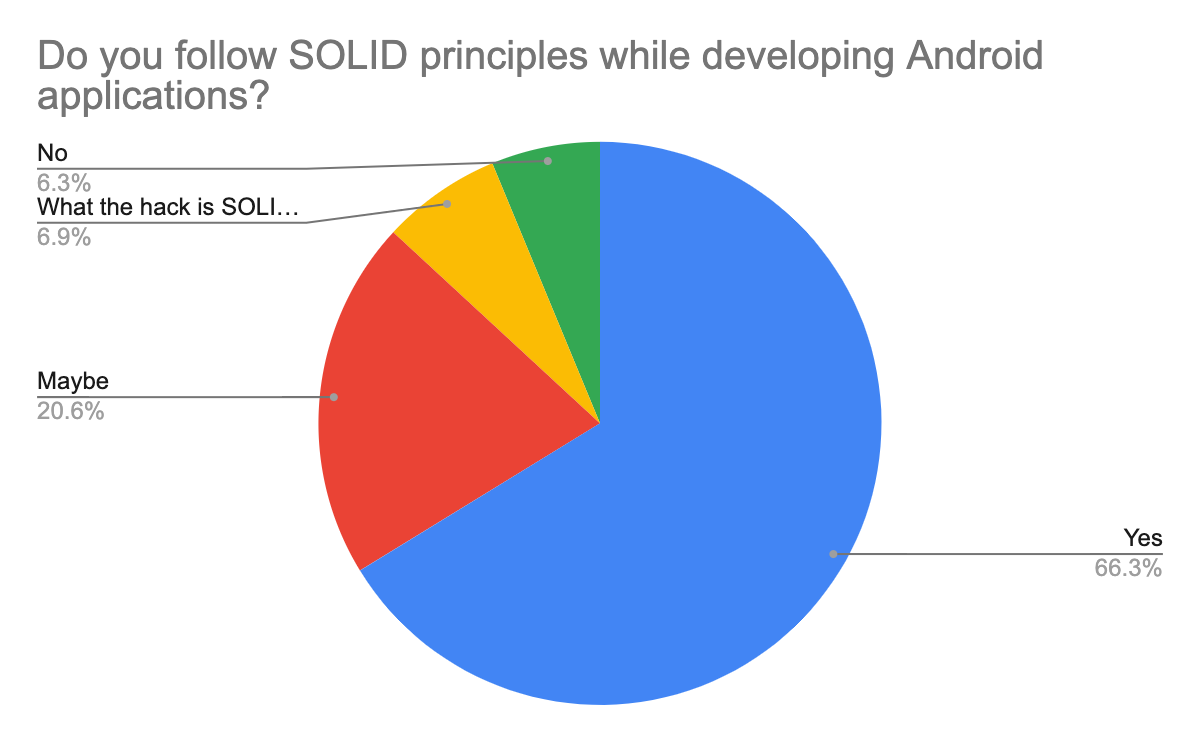
\includegraphics[scale=0.25]{figures/solid.png}
    \caption{SOLID principles usage results}
    \label{fig:solid}
\end{figure}
\FloatBarrier

It is not easy to understand why people who develop software professionally in the Android field or any other field do not want to follow SOLID principles or are not aware of these principles, especially if these people are experienced developers. As stated in chapter 4 before, Mooncascade's Android team actively applies SOLID principles in Android application development processes. This selection is compatible with general Android developer behaviour, as can be seen in the results above.

In the 6th question of the questionnaire, the participants were asked whether they apply the "Clean Code" principles while developing Android applications. The starting point, purpose, advantages and disadvantages of these principles are given in section 4 in detail. According to the results, 75\% of the participants stated that they either used or could use these principles. While 13.8\% of the participants stated that they do not use these principles, it was observed that 11.3\% of the participants were not even aware of these principles. The breakdown of the participants’ answers in the form of a pie chart can be seen below in Fig. \ref{fig:clean_code}.
\begin{figure}[ht!]
    \centering
    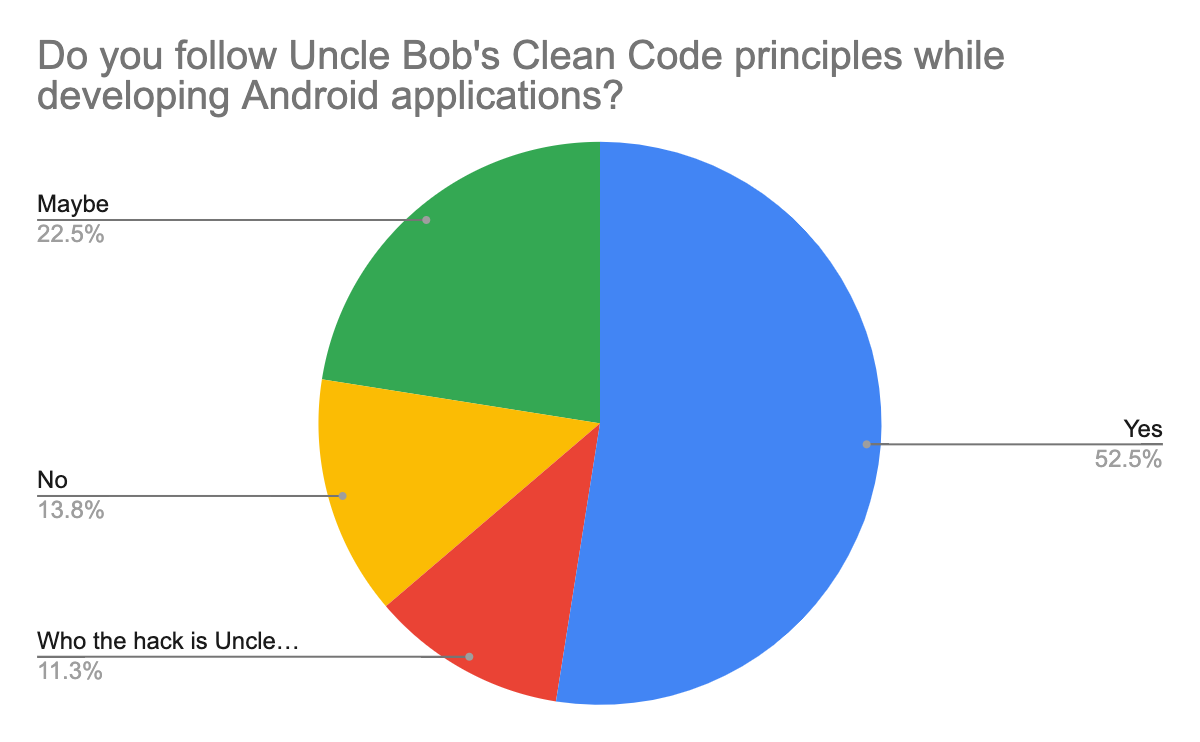
\includegraphics[scale=0.25]{figures/clean_code.png}
    \caption{Clean Code principles usage results.}
    \label{fig:clean_code}
\end{figure}
\FloatBarrier

Although there are many advantages of Clean Code principles, discussions are still going on in Android and other software development communities about Uncle Bob and his principles. From this point of view, it can be understood that although most of them actively use these principles, some developers do not. This situation can be interpreted as applying advanced concepts such as Clean Code or SOLID while developing the software directly proportional to the experience. Mooncascade's Android team mainly applies Clean Code principles in Android application development processes. This selection is compatible with general Android developer behaviour when compared to the results above. Further information about how Mooncascade's Android team applies Clean Code principles can be found in section \ref{section:4.4.2}.